% Nach dem "%"- Zeichen folgt in LaTeX ein Kommentar. Will man das %-Zeichen selber darstellen, hilft \%


%Schriftgröße, Layout, Papierformat, Art des Dokumentes, Zeichenkodierung
\documentclass[11pt,a4paper]{article}
\usepackage{float}
\usepackage{derivative}
\usepackage[T1]{fontenc} % Westeuropäische ASCII-Codierung
\usepackage[utf8]{inputenc} % UTF8-Codierung

%Einstellungen der Seitenränder und Ausschalten der Absatzeinrückung
\usepackage[left=2cm,right=2cm,top=2cm,bottom=2cm,includeheadfoot]{geometry}
\setlength{\parindent}{0ex} % Keine Einrückung der ersten Absatz-Zeile
\setlength{\parskip}{\baselineskip} % Abstand zwischen den Absätzen 
\renewcommand{\topfraction}{1} % Legt den Anteil oben auf der Seite fest, den Abbildungen und Tabellen einnehmen dürfen. 
\renewcommand{\topfraction}{1} % Legt den Anteil unten auf der Seite fest, den Abbildungen und Tabellen einnehmen dürfen.

%neue Rechtschreibung
\usepackage[ngerman]{babel}

%Kopf- und Fußzeile
\usepackage{fancyhdr}
\pagestyle{fancy}
\fancyhf{}

%Höhe der Kopfzeile, muss je nach Fehlermeldung angepasst werden
\setlength{\headheight}{15pt}

% Texte in Kopf und Fußzeile, dies muss man selbst anpassen.
%Kopfzeile links
\fancyhead[L]{Stand: \today}
%Kopfzeile mittig
\fancyhead[C]{Physikalisches Prkatikum: Zustandsgleichung realer Gase}
%Kopfzeile rechts
\fancyhead[R]{Seite \thepage}
%Linie oben
\renewcommand{\headrulewidth}{0.5pt}

%Linie unten
\renewcommand{\footrulewidth}{0.5pt}

%Weitere Packages
\usepackage{siunitx}
\usepackage{amsmath} %Mathemodus
\usepackage{amsfonts} %Matheschriften
\usepackage{amssymb} %Mathesymbole
\usepackage{mathptmx} % Einstellung für Schriften und Sonderzeichen in mathematischen Umgebungen
\usepackage{wasysym} % Stellt diverse Sonderzeichen bereit

\usepackage{graphicx} %Grafiken

\usepackage{multirow}


\usepackage{color}
\usepackage{colortbl}
\definecolor{gray}{gray}{0.75}
\definecolor{gray5}{gray}{0.5}

%Formatierung der Bildunterschriften und Tabellenüberschriften
\usepackage{caption}
\captionsetup{format=hang,labelfont=it,textfont=it} % Einrücken von Bildunterschriften, kursiver text

% Hier beginnt dann das eigentliche Dokument.
\begin{document}

% Erzeugen des Titels mit Namen und Datum. Die erste Seite hat dann keine Kopf- und Fußzeile
\title{Physikalisches Praktikum: Zustandsgleichung realer Gase}
\author{Nehir Şen  \\
        Kostiantyn Shchurovskyi \\ \\
        Jan Schmidbauer
        Kurs 4, Team 8-9}
\date{\today}
\maketitle

% Erzeugen des Inhaltsverzeichnisses
\tableofcontents


% Neue Seite
\clearpage

% Erster Abschnitt
\section{Einleitung}
In diesem Praktikum wurden Versuche zur Thermodynamik der realen Gasen(und Flüssigkeiten) gestellt.
\section{Grundlagen}
Zustandsgleichung für ideale Gleichung lautet:
\begin{equation}
    p\cdot V = n\cdot R\cdot T = N\cdot k_B\cdot T \label{eq:ideal}
\end{equation}, wobei $p$ in \unit{Pa} Druck, V in \unit{m^3} Volumen, $n$ in \unit{mol} die Stoffmenge, $T$ in \unit{K} die Temperatur, $R =$ \qty{8,314462618}{\frac{J}{mol.K}} die universelle Gaskonstante, $N$ Anzahl der Teilchen und $k_B$ \qty{1,380649e-23}{\frac{J}{K}} sind. Darüber hinaus gilt die Gleichung $R = k_B \cdot N_A$, wobei $N_A =$ \qty{6,02214076e-23}{\mol^{-1}}.

Außerdem verwendet man die Bezeichnungen $M = \frac{m}{n}$ für molare Masse und $V_m = \frac{V}{n} = \frac{R\cdot T}{p}$ für molares Volumen.

Für die realen Gasen verwendet man die Gleichung~\eqref{eq:real}
\begin{equation}
    \left(p + \left(\frac{n}{V}\right)^2\cdot a\right)\cdot\left(V - b\cdot n\right) \label{eq:real}
\end{equation}, wobei $a$ und $b$ konstant für ein Gas ist.

Auf der Abb.~\ref{fig:IsoVan} sind Isothermen(Daten mit gleicher Temperatur) für ein Van-der-Waals Gas dargestellt. Es gibt nur einen Punkt $(p_\text{krit}, T_\text{krit}, V_\text{krit})$ für jeden $n$, der sogenannte kritischer Punkt, sodass $\left(\pdv{p}{V}\right)_{(p_\text{krit}, T_\text{krit}, V_\text{krit})}$ und $\left(\pdv[2]{p}{V}\right)_{(p_\text{krit}, T_\text{krit}, V_\text{krit})}$ gleichzeitig $0$ sind:
\begin{gather}
    V_\text{krit} = 3\cdot b\cdot n \label{eq:Vkrit} \\
    p_\text{krit} = \frac{a}{27b^2} \label{eq:pkrit}
\end{gather}

\begin{figure}
    \centering
    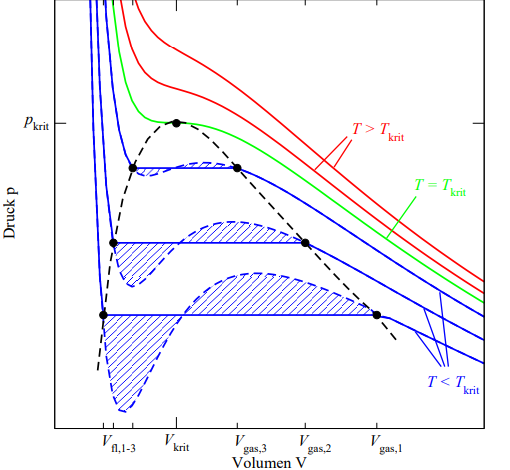
\includegraphics[width=0.8\linewidth]{ZUS/Screenshot Van der Waals.png}
    \caption{Van-der-Waals Isothermen, \cite{ZUS}}
    \label{fig:IsoVan}
\end{figure}

Auf der Abb.~\ref{fig:IsoVan} verhalten sich Isothermen für $T<T_\text{krit}$ nicht auf dem ganzen Bereich so, wie es Gleichungen darstellen. In diesem Bereich findet ein Phasenübergang von Flüssigkeit zu Gas(Koexistenz von Gas und Flüssigkeit) statt. Dabei ist der Druck konstant(temperaturabhängig) und ist so ausgewählt, dass die gestrichenen Flächen den gleichen Flächeninhalt haben. Der Druck heißt Dampfdruck $p_d$ Für $T>T_\text{krit}$ existiert die Substanz nicht in flüssiger Form.

Clausius-Clapeyron-Gleichung gibt Verhalten von $p_d$ an:
\begin{equation}
    \odv{p_d}{t} = \frac{L}{T\cdot (V_g - V_{fl})}
\end{equation}, wobei $L$ die Verdampfungsenthalpie, $V_g$ das Volumen an der Grenze zwischen Gas und Koexistenz und $V_{fl}$ das Volumen an der Grenze

\section{Experimentelles Vorgehen}

\section{Ergebnisse} 

\section{Diskussion}

\section{Zusammenfassung}



%\section{Anhang}

\section{Literaturangaben}

\begin{thebibliography}{Ddddd} 

\bibitem{ZUS}{Anleitung zum Versuch ZUS, im Moodle Kurs}

\bibitem{Vorlage}{LaTex Vorlage für Praktikum in Moodle Kurs}

\bibitem{ABW}{Hinweise zur Beurteilung von Messungen, Messergebnissen und Messunsicherheiten; im Moodle Kurs}

\end{thebibliography}

\end{document}
